Sowohl für das Backend als auch für das Frontend wurde jeweils ein 
eigenes Dockerfile erstellt. Beide verwenden Multi-Stage Builds, 
was bedeutet dass der Build-Prozess und die finale Ausführungsumgebung 
voneinander getrennt sind. Das Ergebnis sind kleinere Images, da 
Build-Werkzeuge wie Maven oder Node.js nicht im fertigen Image 
landen.

\subsubsection{Frontend}

Das Frontend-Dockerfile besteht aus zwei Stages. 
Abbildung~\ref{fig:dockerfile-frontend} zeigt das vollständige 
Dockerfile.

\begin{figure}[H]
    \centering
    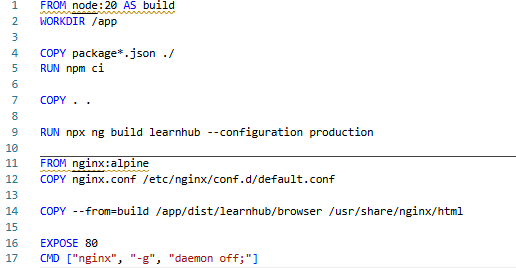
\includegraphics[width=0.75\textwidth]{pics/dockerfileFrontend.png}
    \caption{Dockerfile des Frontends}
    \label{fig:dockerfile-frontend}
\end{figure}

In der ersten Stage wird Node.js verwendet um die Angular-Anwendung 
zu bauen. Dabei werden zuerst nur die \texttt{package.json} Dateien 
kopiert und die Abhängigkeiten installiert. Der Grund dafür ist 
simpel: Abhängigkeiten ändern sich viel seltener als der eigentliche 
Code. Docker merkt sich diesen Schritt im Cache, sodass bei den 
meisten Builds die Abhängigkeiten nicht erneut heruntergeladen 
werden müssen. Das spart Zeit. Erst danach wird der restliche Code 
kopiert und die Anwendung gebaut.

In der zweiten Stage wird Nginx als Webserver verwendet. Hier 
landet nur das fertige Build-Ergebnis aus der ersten Stage, also 
die fertigen HTML, CSS und JavaScript Dateien. Node.js und alle 
anderen Tools die zum Bauen gebraucht wurden sind im finalen 
Image nicht mehr vorhanden. Zusätzlich wird eine angepasste 
Nginx-Konfiguration kopiert, die sicherstellt dass das Routing 
der Angular-Anwendung korrekt funktioniert.

\subsubsection{Backend}

Das Backend-Dockerfile funktioniert nach demselben Prinzip, 
verwendet aber Maven und Java statt Node.js. 
Abbildung~\ref{fig:dockerfile-backend} zeigt das vollständige 
Dockerfile.

\begin{figure}[H]
    \centering
    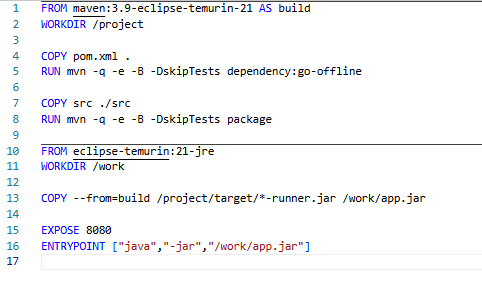
\includegraphics[width=0.75\textwidth]{pics/dockerfileBackend.png}
    \caption{Dockerfile des Backends}
    \label{fig:dockerfile-backend}
\end{figure}

In der ersten Stage wird Maven verwendet um die Quarkus-Anwendung 
zu kompilieren. Auch hier wird das Caching gezielt genutzt: Zuerst 
wird nur die \texttt{pom.xml} kopiert und alle Maven-Abhängigkeiten 
heruntergeladen. Da sich diese selten ändern, muss dieser Schritt 
bei den meisten Builds nicht wiederholt werden. Danach wird der 
Quellcode kopiert und die Anwendung gebaut. Tests werden dabei 
bewusst übersprungen, da diese in einer eigenen Pipeline laufen.

In der zweiten Stage wird nur die Java Runtime verwendet, also 
das Minimum das zum Ausführen der fertigen Anwendung gebraucht 
wird. Aus der ersten Stage wird nur das fertige JAR-File 
übernommen und beim Start des Containers automatisch ausgeführt. 
Maven und das vollständige JDK sind im finalen Image nicht mehr 
enthalten, was das Image deutlich kleiner macht.

\subsubsection{Vergleich der beiden Dockerfiles}

Beide Dockerfiles folgen demselben Muster aber sind auf ihre 
jeweilige Technologie zugeschnitten. Was sie gemeinsam haben 
ist das Dependency-Caching und die Trennung von Build und 
Ausführung. Der Unterschied liegt nur in den verwendeten 
Technologien, Node.js und Angular auf der einen Seite, 
Maven und Quarkus auf der anderen.